\chapter{Calico}

% [anticpated/actual features]
% [purpose, how does it work]
% [supports designers in sketching]

\section{Canvas and Grid}

% http://en.wikibooks.org/wiki/LaTeX/Floats,_Figures_and_Captions
\begin{figure}[htb]
\centering
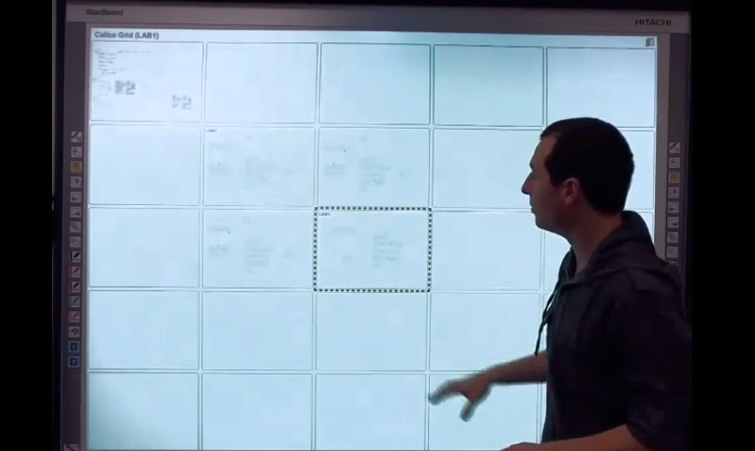
\includegraphics[width=0.8\textwidth]{grid.jpg}
\caption{The grid view within Calico}
\label{fig:grid}
\end{figure}
%The grid is the focal point of any session in Calico.
%It shows the various canvases that users may interact with in a given session.
%Users may perform various operations on canvases from the grid, such as duplicating or clearing individual cells.
%The grid also gives a clear overview of the designs that are happening in a session.

\todo{From Andre}
Calico as a drawing tool, is centered on the metaphor of canvases, with the grid acting as the focal point.
It has a mulitude of canvases organized in a grid. [See Figure \ref{fig:grid}]
Users can draw in each of these canvases.
Each of these canvases can contain sketches, writings, or anything that the designer desires.
Because these canvases are organized in a grid, users are able to move from one canvas to another in one of two ways: They can switch to a ``grid view'' that gives them an overview of all the cell, or they can use the white navigation tabs located on the side that will allow them to jump to the adjacent canvas.
The gray tabs allow the designer to ``branch off'' and create a copy of the current canvas, but in another cell, so that the two can be easily compared.

\section{Gestures}
As a drawing tool, gestures are an integral part of Calico.
Gestures allow users to easily perform operations by performing a defined action with the mouse.
In the original version of Calico, there were many different gestures that users could perform.
In order to allow scraps to be easily removed without requiring a break in the user's thought process, we opted to allow users to ``strike-through'' a scrap with a sketching gesture, which would immediately erase the scrap and it's contents.
As a diagramming tool, users were constantly linking scraps to show inheritance, abstraction, etc.
Due to this constant linking, we created a gesture that would allow users to draw a line from one scrap to another, and Calico would automatically turn this into a directed arrow.
Once two scraps were ``linked,'' the arrow would be anchored to them, and would follow the scrap whenever it was moved on screen.
Another gesture that was added was the ability to ``enlarge'' a scrap by drawing a ``blister'' or bubble on the edge of the scrap.
By drawing this extra bubble, the scrap area would be enlarged to equal the size of the bubble that was just drawn.


\section{Scraps}
Scraps in Calico can be thought of as ``scraps of paper'' that one would place on a desk or on a white board.
Scraps keep their shape -- whatever the designer draws, this shape will be kept throughout the design phase.
However, scraps are manipulatable in many different ways -- they are stackable, removable, relatable, movable. 
\todo{Add image showing one of these ways}
In the original version of Calico, all scraps have a ``dot'' that acts as a menu where various actions can be performed on the scrap itself.
Designers tend to use many different notations when they are designing, and we want designers to be able to sketch in the notations that they are most comfortable with, but we also want to be able to work with their designs.
Our goal is to be able to interact with the designers so that they are able to manipulate the objects, but we do not want to be intrusive in the way a formal design tool would be.

We created scraps as the answer to allowing the content of a sketched design to become ``active'', while still allowing the designer to be completely free in their design and still able to manipulate their sketches.
The key is that we leave them in the same shape they were in when they were drawn, but that they become ``active''. 
Anything drawn on top of that scrap automatically comes associated with the original scrap.
Designers can relate scraps with each other simply by drawing a line from one to the other, which would be converted to a directional arrow, linking the two scraps with each other.
\todo{Put a picture of a drawing with some arrows and stuffit}
%Scraps can be easily relocated to different parts of the screen, or even other canvases.
%Scraps can be stacked on top of each other and then treated as a unit or group.
%By treating scraps as if they were pieces of paper, we [make it easy to understand the manipulation], as designers can easily relate Calico to their current design 

\section{Palette}
The palette in Calico provides users with a ``drawer'' that can easily be used to store commonly used shapes and artifacts.
The palette can be synchronized across sessions so that other users in the session can share the same palette.